\documentclass[]{article}
\usepackage{geometry}
\geometry{
	a4paper,
	total={170mm,257mm},
	left=0.75in,
	top=0.75in,
	right=0.75in,
	bottom=1in,
}
\usepackage{gensymb}
\usepackage{lipsum}
\usepackage{graphicx}
\usepackage{caption}
\captionsetup{width=0.8\textwidth, justification=centering}
\usepackage{amsmath}
\usepackage[url=false,
backend=bibtex,
style=authoryear-comp,
doi=true,
isbn=true,
backref=false,
dashed=false,
maxcitenames=2,
maxbibnames=99,
natbib=true]{biblatex}
\addbibresource{bubbleBurstingVE.bib}
\DeclareNameAlias{author}{last-first}
\renewbibmacro{in:}{}
\usepackage{xcolor}
\usepackage[colorlinks,citecolor=blue]{hyperref}
\DeclareFieldFormat[article, inbook]{title}{#1}

\usepackage{fancyvrb}

\title{\textbf{Reply to Refree 3}}
\date{\vspace{-5ex}}
\newcommand{\AKD}[1]{{\textcolor{magenta}{#1}}}

\usepackage[textwidth=\dimexpr\textwidth-2cm\relax]{todonotes}
\makeatletter
\@mparswitchfalse%
\makeatother
\normalmarginpar %for right-handed notes and lines, or
\newcommand{\vsy}[1]{\todo[color=orange, bordercolor=none, textcolor=white]{Vatsal}\textcolor{orange}{#1}}

\newcommand{\oo}{\color{magenta} \normalfont}
\newcommand{\bb}{\color{black} \normalfont}

\newcommand{\vs}{\color{orange} \normalfont}

\renewcommand{\thefigure}{R3.\arabic{figure}}
\captionsetup[figure]{labelformat=default}

\begin{document}

	\maketitle % This command prints the title, author, and date
We thank the referee for carefully reading our manuscript and providing valuable feedback and suggestions. We have reviewed the referee’s comments and made changes based on their suggestions. Below, we offer a point-to-point reply to each of the referee’s comments and include the changes made in the manuscript. The referee’s comments are in italics, and our replies are in plain black. Changes in the manuscript are highlighted in magenta.

\begin{enumerate}
    \item \textit{I think the paper is well constructed, the subject is interesting, the study is serious and Ice can be confident in their results. I think it should eventually be published in JFM. However, I find some parts rather hard to read, especially parts 4.1, and 4.2.2, so I recommend redrafting them to make them more readable.}

%  \vsy{ \#TODO-DONE: Again, you cannot say that we agree with the reviewer and then go around in circles. It is okay to disagree with reviewer and take a stand. But, do not mix the two.}

	We have redrafted section 4.1 and 4.2.2 to streamline the discussions:

	\oo
	\S~4:
	The bursting bubble dynamics in viscoelastic media exhibit distinct behavior compared to Newtonian fluids.
	Our analysis reveals three well-defined regimes: (i) jets that form droplets, (ii) jets without droplet formation, and (iii) complete suppression of jets. While viscoelasticity significantly modifies jet dynamics, the capillary wave propagation prior to jet formation remains remarkably unaffected.
	This section explores the transitions between these regimes across the $Ec$-$De$ phase space, extending our earlier analysis of the limiting cases $De \to \infty$ and $De \to 0$ from \S~3.

	\S~4.1:
	The transitions between these regimes depend on both $Ec$ and $De$, exhibiting markedly different characteristics in two limiting cases: $De \to \infty$ and $De \to 0$.
	Figure~7 maps these transitions in the elastocapillary-Deborah number ($Ec$-$De$) phase space, delineating the boundaries between droplet-forming jets and jets without droplets. Figure~8 complements this by illustrating the transition to complete jet suppression. Notably, the infinite $De$ asymptotic behavior extends down to $De \approx 1$, reflecting that polymers lack sufficient time to relax when relaxation times exceed the process timescale.\bb

	For polymeric liquids with long relaxation times ($De \gg 1$), we observe that:

	\begin{enumerate}
		\item the dropping transition occurs at $Ec_d(Oh_s)$, with strong $Oh_s$ dependence (Figures~4b and 7), and
		\item the jetting transition occurs at $Ec_j \approx 0.086$, independent of $Oh_s$ (Figure~8a).
	\end{enumerate}

	Conversely, for polymeric liquids with short relaxation times ($De \ll 1$), we find that both transitions are $Oh_s$-independent and occur at constant polymeric Ohnesorge number $Oh_p = Ec \times De$:

	\begin{enumerate}
		\item the dropping transition occurs at $Oh_{p,d} \approx 0.048$ (Figure~7) and
		\item the jetting transition occurs at $Oh_{p,j} \approx 0.129$ (Figure~8b).
	\end{enumerate}

	\oo
	These behaviors reflect fundamentally different physical mechanisms: at high $De$, depending on $Oh_s$, the medium behaves like an elastic solid ($Oh_s \to 0$) or Kelvin-Voigt solid (finite $Oh_s$). However, at low $De$, polymer addition manifests as an enhanced viscous effect characterized by $Oh_p$.\bb
	We further investigate the jetting transition using slender jet equations in \S~4.2 following similar approaches by \citet{driessen2013stability,gordillo2020impulsive,zinelis2023transition,sen2024elastocapillary}.

	\S~4.2.2:
	\oo
	In the limit of zero $De$ limit, polymeric liquids exhibit additional viscous effects characterized by the polymeric Ohnesorge number $Oh_p$ (also see \S~4.1).
	The maximum elastic stress $\text{max}(\sigma_{p,\text{base}}(t))$, when normalized by the Newtonian-like viscous stress $\sigma_{N,\text{base}}$, collapses for all $Oh_p$ as $De \to 0$, where
	\bb
	\begin{align}
		\sigma_{N,\text{base}} =  \frac{2}{h_{\text{base}}^2}\int_{o}^{h_{\text{base}}} G\lambda\frac{\partial v}{\partial z} h\mathrm{d}h.
	\end{align}

	%\noindent Here, $\eta_p = G\lambda$ \DL{represents the polymeric contribution to the shear viscosity of the polymeric liquid.}
	\oo
	As $De$ approaches unity, marking the onset of the infinite $De$ asymptotic regime, the elastic stress scales as $\text{max}(\sigma_{p,\text{base}}(t)) \sim De \times \sigma_{N,\text{base}}$.
	%we observe a scaling behavior of $\text{max}(\sigma_{p,\text{base}}(t)) \sim De \times \sigma_{N,\text{base}}$.
	This scaling remarkably resembles that predicted by \citet{boyko2024flow} for flow in a slowly varying contraction at the infinite $De$ asymptote, despite significant geometric differences. While our study focuses on free surface flows and \citet{boyko2024flow} examined contraction geometries, this unexpected similarity hints at a potentially universal behavior near the infinite $De$ asymptote. To further examine this intriguing connection, a similar closed-form $De$ expansion for free surface flows is necessary. However, we caution that this scaling approach to the infinite $De$ asymptote could be system-dependent \citep{hinch2024fast}.

	At zero $De$, the elastic stress reduces to a Newtonian-like viscous stress with polymeric viscosity $\eta_p$, yielding $\sigma_p \approx 2G\lambda\boldsymbol{\mathcal{D}}$ for Oldroyd-B rheology. The force balance in equation~(4.2) becomes
	\bb
	%Here, we focus at the zero $De$ limit, where the elastic stress can be replaced with a Newtonian-like viscous stress with polymeric viscosity $\eta_p$ such that the \VS{jetting} transition occurs at constant polymeric $Oh_p$.
	%The polymeric stress contribution becomes $\sigma_p \approx 2G\lambda\boldsymbol{\mathcal{D}}$ (for the Oldroyd-B rheology, see also equation~\eqref{oldroydb}).
	%Consequently, we can rewrite the force balance in equation~\eqref{forcebalance} as

	\begin{align}
		\frac{d \mathcal{M}_\text{jet}}{d t} = \left(3\eta_s + 2G\lambda\right)h^2\frac{\partial v}{\partial z}\Bigg|{\text{base}},
		\label{etaeffect}
	\end{align}

	\noindent which depicts the balance of jet inertia with viscous forces.
	\oo Using characteristic scales for jet momentum $\mathcal{M}_{\text{jet}} \sim \rho V_\text{jet} h_{\text{base}}^3$, velocity gradient $\partial_zv \sim V_{\text{jet}}/\delta_\eta$, and time $\tau_i \sim h_{\text{base}}/V_\text{jet}$, the force balance yields\bb

	\begin{align}
		\rho V_{\text{jet}}^2 \sim \eta_{\text{effective}}\frac{V_{\text{jet}}}{\delta_\eta}.
		\label{scaling}
	\end{align}

	\noindent Here, $\delta_\eta$ represents the viscous length scale and the effective viscosity is

	\begin{align}
		\label{eqn:etaEff}
		\eta_{\text{effective}} = 3\eta_s + 2G\lambda .
	\end{align}

	\noindent \oo Since polymers do not affect the flow before jet formation (\S~3), the jet Weber number remains constant at inception \citep{blanco2021jets},\bb

	\begin{align}
		We_{\text{jet}} = \frac{\rho V_{\text{jet}}^2 \delta_\eta}{\gamma} =\,\text{constant}.
		\label{We}
	\end{align}

	\noindent Combining equations \eqref{scaling} and \eqref{We}, we get

	\begin{align}
		V_{\text{jet}}  \sim \frac{\gamma}{\eta_{\text{effective}}}
		\label{velocityscale}
	\end{align}

	\noindent \oo analogous to Newtonian media but with modified viscosity \citep{gordillo2019capillary, blanco2020sea}.\bb


    \item \textit{I am not convinced by the use of Lmax as an observable and I think the authors should plot the nondimensional velocity of the jet as defined in Fig11b.}

    We appreciate the reviewer's suggestion regarding the jet velocity as an observable. Indeed, jet velocity is an important characteristic of the bubble-bursting process, and we have included detailed velocity analysis in our study, particularly in Section 4.2.2 and Figure 11(b). However, we chose $L_{\text{max}}$ as our primary observable for several reasons:

    \begin{itemize}
    	\item The jet velocity varies significantly with time during the process (as noted by several studies, including \citet{deike2018dynamics,gordillo2019capillary}), making it necessary to choose a specific definition or time point for measurement (see appendix A of \citet{sanjay2021bursting} for a detailed comparison). In contrast, $L_{\text{max}}$ provides an unambiguous, well-defined maximum value that clearly characterizes the jet evolution. Importantly, $L_{\text{max}} = \int_{t_i}^{t_f}v_{\text{jet}}(t)dt$, where $t_i$ and $t_f$ are the inception time and time at $L_{\text{jet}} = L_{\text{max}}$, respectively, showing that $L_{\text{max}}$ inherently captures the complete velocity history of the jet.

    	\item In our study, we found that for a wide range of $Ec$ and $De$, the jet velocity remains close to Newtonian values, particularly during the initial stages when shear dominates the flow. This is because polymeric effects become significant primarily during elongational flow, which develops later in the process. The jet length $L_{\text{max}}$, by integrating over the entire process, captures these later-stage polymeric effects more effectively, making it a more suitable metric for mapping the regime transitions.

    	\item In the `Drops' regime, we observe that the jet velocity exhibits an inverse relationship with droplet size, following the known scaling \citep{blanco2020sea} where smaller drops are ejected at higher velocities. This relationship is captured in our analysis through both $L_{\text{max}}$ and the detailed velocity scaling presented in Section 4.2.2.

    	\item While using $L_{\text{max}}$ as our primary observable, we have conducted comprehensive velocity analysis throughout the paper. Section 4.2.2 demonstrates that velocity follows $V_\text{jet} \sim \gamma/\eta_\text{effective}$ with a modified effective viscosity (Figure 11b). This velocity analysis complements our regime mapping based on $L_{\text{max}}$.

    \end{itemize}

    \item \textit{The authors show that rising elastic stresses suppress droplet formation (Fig4b), surprisingly for Ohs around $2 \times 10^{-3}$, rd seems to have a non-monotonic variation, can the authors give details on this point?}

    We thank the reviewer for their observation. We would like to clarify that $r_d$ exhibits a monotonic decrease with $Oh_s$--in fact, it remains invariant for $Ec \to 0$, and decreases when very close to the transition.
    The apparent non-monotonic behavior around $Oh_s \approx 2 \times 10^{-3}$ is probably an artifact of visual interpretation, particularly in the transition region.
    We have thoroughly verified the monotonous nature of these variations in our numerical data. To enhance clarity and prevent potential misinterpretation, we have moved the regime labels (Drops and No-drops) outside of the colormaps in the revised figures. This modification allows for better visualization of the continuous variation in $r_d$ across the phase space (see figures~\ref{highDe} and~\ref{smallDe}).

    \begin{figure}
    	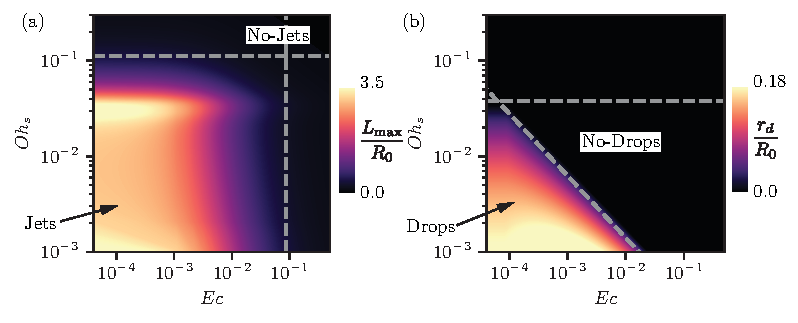
\includegraphics[width=\textwidth]{../Main/High_De_05-eps-converted-to.pdf}
    	\caption{(a) The maximum jet length $L_{\text{max}}$ at $De \to \infty$ in the $Ec$-$Oh_s$ phase space, depicted by the colormap, where the lighter region corresponds to higher values. For the Newtonian liquid $\left(Ec \to 0\right)$, the jetting transition occurs at $Oh_s = 0.11$, denoted by the horizontal dotted line. Due to the elastic effects, this transition occurs at $Ec = 0.086$, as depicted by the vertical dotted line. (b) The size of the first droplet at $De \to \infty$ in the $Ec$-$Oh_s$ phase space. For the Newtonian liquid, the dropping transition is observed at $Oh_s = 0.0375$, denoted by the horizontal dotted line. Further, the transition due to elastic effects is very sensitive to $Oh_s$ and is shown by the inclined dotted line.}
    	\label{highDe}
    \end{figure}

	\item
	\begin{itemize}
		\item \textit{Fig 6b: the Ohs-independent transition due to elastic effects occurring at Ec = 2.5 is very abrupt (much more than in Fig 4(b) for example), can the authors elaborate on this surprisingly violent variation?}

		%    \vs
		%    Indeed, the transitions at $De = 0.01$ shown in Figure 6(b) are abrupt compared to the elastic case ($De \to \infty$) shown in Figure 4(b). We speculate the reason behind the different nature of transition in both cases. At small $De$, the medium has a viscous-like response, and as $Ec$ increases, close to the critical value, the jet width reduces sharply (see Figure 12(b)), and upon further increasing droplets are no longer produced. However, at high $De$, waves are not affected, instead, the droplets are suppressed because of the elastic effects during the jetting (after the collapse of capillary waves). We speculate that this is the reason, why at high $De$, the transition occurs over a wider range of $Ec$, compared to cases at small $De$ where the transitions are abrupt.
		%    \bb
		%
		%    \vsy{\#TODO-done: in the very next comment you say that there was a post processing glitch in 6b. In your new figure 6b. the transition is not abrupt.}

		\item \textit{Why do not we see the expected minimum drop size at the singularity in Fig 6b?}

	\end{itemize}

   We thank the reviewer for their careful observation regarding the transitions shown in Figure 6(b). Upon re-examining our data, we identified and corrected a post-processing bug that led to an artificially abrupt transition at Ec = 2.5. The revised Figure 6(b) now accurately represents the data, showing:

   \begin{itemize}
   	\item A gradual transition between the drop and no-drop regimes, similar to the behavior seen in Figure 4(b)
   	\item The expected minimum drop size near the transition point, which was obscured in the original figure. This minimum drop size is consistent with the minimum jet radius reported in figure 12(b).
   	\item A smooth variation in drop size as Ec increases.
   \end{itemize}

   The corrected figure provides a more complete picture of how the droplet size varies with both $Oh_s$ and $Ec$ in the low De regime. The transition remains $Oh_s$-independent but follows the expected behavior: increasing elastic effects progressively modify the drop formation process rather than causing an abrupt cutoff. We have included this corrected figure in the revised manuscript (see figure~\ref{smallDe}).

    \begin{figure}
   	\centering
   	\includegraphics[width=\textwidth]{../Main/Small_De_05-eps-converted-to.pdf}
   	\caption{(a) The maximum jet length $L_{\text{max}}$ at $De = 0.01$ in the $Ec$-$Oh_s$ phase space, depicted by the colormap, where the lighter region corresponds to higher values. For the Newtonian liquid, the jetting transition occurs at $Oh_s = 0.11$, denoted by the horizontal dotted line. Due to the elastic effects, this transition occurs at $Ec = 9.3$, as depicted by the vertical dotted line. (b) The size of the first droplet at $De = 0.01$ in the $Ec$-$Oh_s$ phase space. For the Newtonian liquid, the dropping transition is observed at $Oh_s = 0.0375$, denoted by the horizontal dotted line. Further, the $Oh_s$-independent transition due to elastic effects occurs at $Ec= 2.5$, as shown by the vertical dotted line.}
   	\label{smallDe}
   \end{figure}

    \item \textit{Fig 7 and 8a: can we predict the quantitative transition value of De between $De^{-1}$ et $De^0$ ?}

    The transition between scalings ($De^{-1}$ to $De^0$) can be understood by comparing the characteristic timescales of the system. The critical Deborah number $De_c$ marking this transition emerges when the polymer relaxation timescale matches the process timescale. Since elastic effects minimally influence the initial shear flow, the jet Weber number remains constant at $We_{\text{jet}} \equiv \rho V_{\text{jet}}^2 \delta_\eta/\gamma \sim \mathcal{O}(10)$ \citep{blanco2021jets}. The transition should occur when the Weissenberg number $Wi \equiv De\sqrt{We_{\text{jet}}} \sim \mathcal{O}(1)$, suggesting $De_c \sim \mathcal{O}(0.1)$.

    This prediction aligns with our numerical observations of elastic stress evolution (Figure 10a), where stresses approach their asymptotic $De \to \infty$ values around $De \approx 0.1$. However, we caution that these are only order-of-magnitude estimates, as the transition likely spans a range of Deborah numbers rather than occurring at a sharp critical value. The uncertainty in precisely determining $We_{\text{jet}}$ also contributes to the approximate nature of this prediction.


    We have added the following to the revised manuscript:

    \oo
    Below this, for $De \sim \mathcal{O}(0.1)$, we observe a transition in scaling behavior, consistent with the Weissenberg number criterion $Wi \equiv De\sqrt{We_{\text{jet}}} \sim \mathcal{O}(1)$, where $We_{\text{jet}}$ is the jet Weber number (equation~(4.8)) that remains approximately constant due to negligible elastic effects during the initial shear flow.
    \bb


    \item \textit{Could the authors describe in greater detail how polymer additives can enhance aerosol production?}

    We thank the reviewer for seeking this clarification and acknowledge that our original phrasing ``potentially enhancing or suppressing aerosol production'' was imprecise and open to interpretation. The effect of polymer additives on droplet formation is nuanced and depends on their concentration and properties. The enhancement or suppression of aerosol production occurs through two distinct mechanisms:

    \begin{itemize}
    	\item At intermediate polymer concentrations (moderate values of Ec and De), we observe that while some jets that would normally form larger droplets (for Newtonian fluids) are suppressed, those that do form can produce smaller droplets compared to Newtonian fluids. This effect is particularly evident in our results showing the transition between different regimes in the $Ec$-$De$ phase space. These smaller droplets can achieve higher velocities and potentially travel greater distances.

    	\item However, increasing polymer concentration beyond certain thresholds will ultimately suppress aerosol production entirely, as clearly demonstrated in our phase diagrams (Figures 12 and 13).
    \end{itemize}

    To better reflect this dual nature, we have modified the relevant text in the conclusion to read:

	\oo
	The results highlight how polymer additives can dramatically alter spray formation, with intermediate values of $Ec$ and $De$ leading to smaller and faster droplets, whereas high values of $Ec$ and $De$ suppress droplet formation entirely \citep{kant2023bag}.
	\bb

	This modification maintains consistency with our abstract's current statement about intermediate polymer concentrations while providing greater clarity about the mechanism of enhancement. It also aligns with our detailed phase space analysis showing the transitions between different regimes of droplet formation.


\end{enumerate}

\printbibliography
\end{document}
